\chapter{Metodology}
\label{chap:Metodology}

About the python algorithm to turn the experiment autonomous it was made a study and modelling of the software architecture to optimize it for further control loop application to be implemented. From the changes made until now it highlights:

- Integrate high speed camera to the experiment routine.

- Remodel the software to support threads in order to separate the sensoring and controlling routines.

- Reduce the data collected size.

- Synchronize the power supply step commands and voltage sensoring.

- Reestructure the setup file in order to make it more intuitive to use the experiment.

- Improvements in code organization and readability.

About the setup,integrate was changed the liquid, nozzle diameter and distance to the plate in order to
make the experiment the most stable and easy to reach cone-jet mode as possible. For example, while doing experiments we discovered that the frequency of the pump machine internal motors was creating an interference in the flowrate. Therefore compromising the stabilization in cone jet mode. A solution for that was to increasethe flowrate wich smooths this pumping noise. For that was also necessary to increase the nozzle diameter to balance with all other variables from the experiment.

\subsection{Pump Integration}

    The pump integration in the automation algorithm bring us a new controllable variable, the Flowrate. Now we can control the spraying mode with the
    two main variables that afect the system. 
    It will bring more complexity for the system since now we are dealing with multivariable control.
    Controlling also the flowrate gives to this project a new dimension in the system giving us freedom to explore the flowrate properties.
    % Our control model is now a MISO \footcite{MISO: Multiple Inputs Single Output} system. The crossover (couple) between the controlled variables will be evaluated in further reports.

    About the pump interface. As I could not find a good ready-to-use library for this pump I developed an simple and intuitive interface to be our software routine.
    The communication protocol used is RS-232. In the software routine the communication used is python serial interface. The pump commands list were found in the user manual.

    \begin{figure}[H]
        \centering
        \resizebox{150mm}{!}{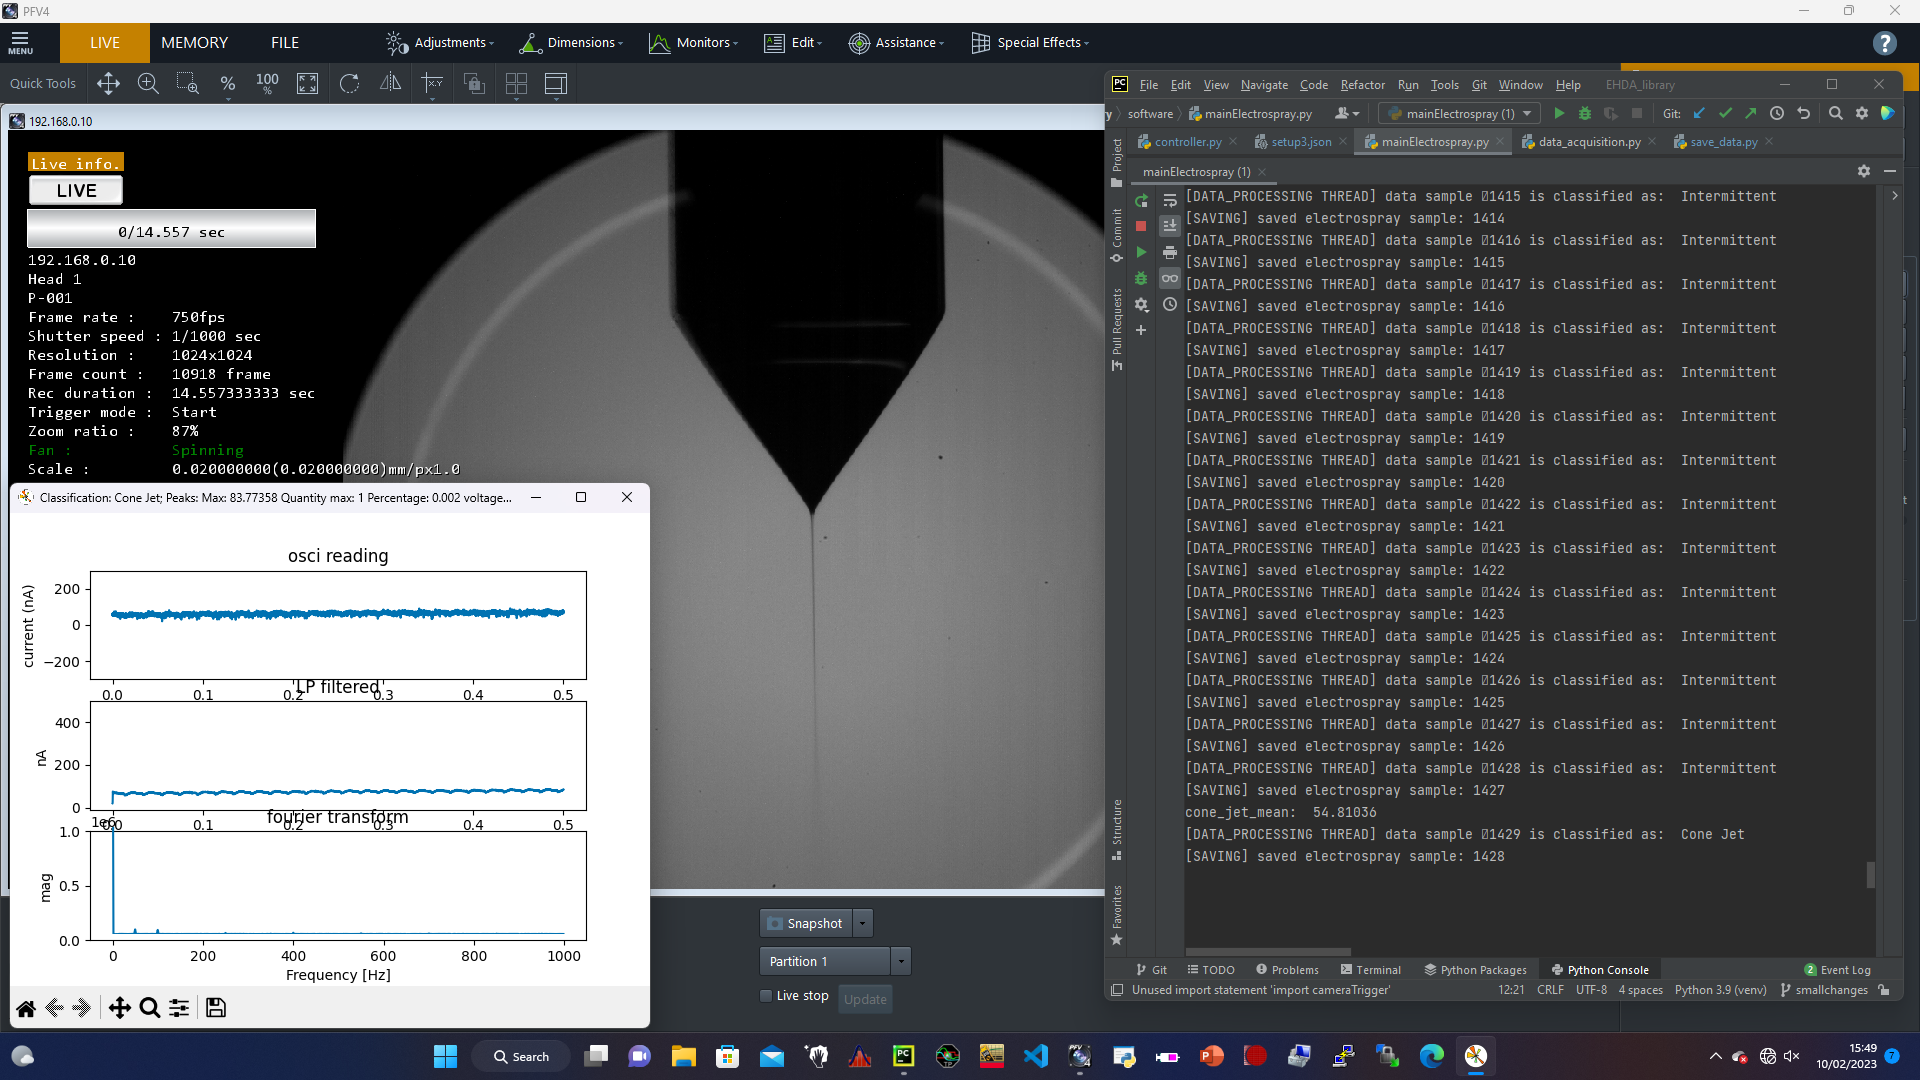
\includegraphics{Figuras/report4/experiment_print1.png}}
        \caption{EHDA automation system setup}
        \label{fig:metodology_example1}
    \end{figure}

\section{System Model}
\label{sec:control_model}


ilustramos o processo com a Figura \ref{fig:control_model_fig}. 

\begin{figure}[H]
  \centering
  \resizebox{150mm}{!}{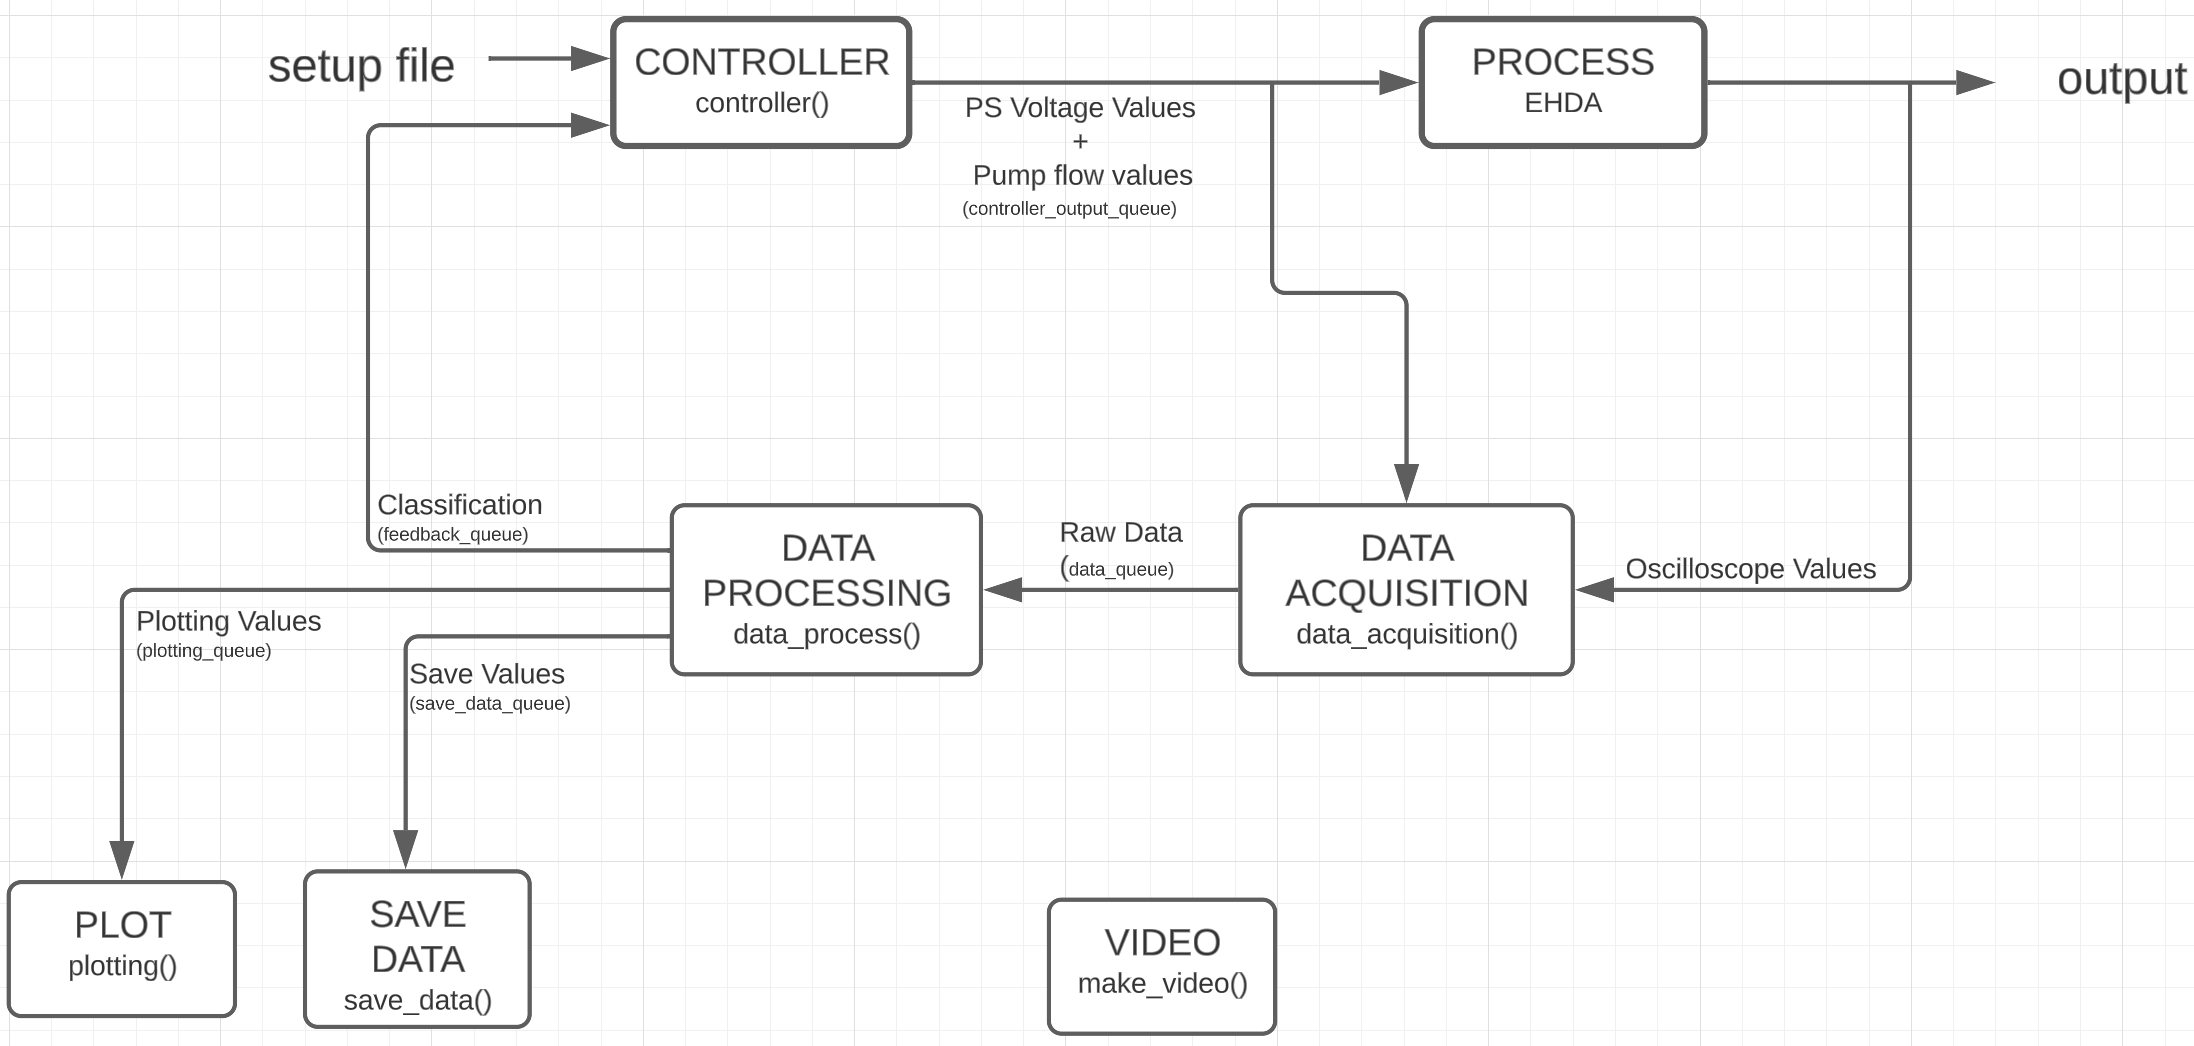
\includegraphics{Figuras/control_loop.png}}
  \caption{EHDA automation system setup}
  \label{fig:control_model_fig}
\end{figure}

\section{Threading and Queues}
\label{sec:concurrency}

    In order to implement this system model to the software and explore parallel processing each system in the
    model was developed as a separate Thread.
    For cuncurrency on flux of data beetween threads was used queues structures.
    A queue is an abstract data type that holds an ordered, linear sequence of items. You can describe it as a first in, first out (FIFO) structure.

    \subsection{Controller Thread}

        It is responsible of sending the power supply set voltage values and the syringe pump the flow rate set values according to the sequence selected.
        Also responsible of sending the finish event command that end the routine and trigger the threads to close their routines.
        As input we have the setup config file and the \emph{feedback\_queue}. As output we have the values in the emph{controller\_output\_queue()}.

    \subsection{Data Acquisition Thread}

        It is responsible for reading the current data from the oscilloscope, humidity and temperature data from the DHT11 sensor, voltage from the powersupply, flowrate from the pump and concatenate into one sample data.
        As output we have the values in the emph{data\_queue()}.

    \subsection{Data Processing Thread}

        It is responsible for calculating the statistical values from the raw data and classify it in the respective spray mode for that sample.
        As output we have the values in the emph{save\_data\_queue()}, emph{plotting\_queue()} and emph{feedback\_queue()}.
    
        \subsection{Save Data Thread}

        After the processing the data is saved in real time in a json file using \emph{jsonstreams} library to save one sample structure at a time.

        With the new streamming model of saving a new structure of the collected data were created.
        Instead of having all data measurements values and after all data processing values we now are saving for each sample the measurements and processing values.
        The structure of the 
    
        \begin{figure}[H]
            \center
            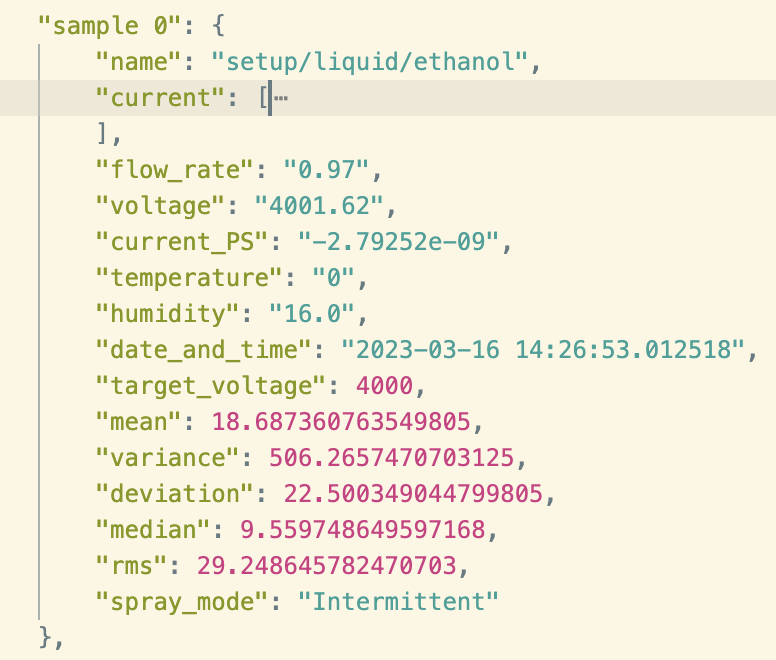
\includegraphics[width=10cm]{Figuras/19:03/new_sample.png}
            \caption{Output data json structure}
        \end{figure}
    
        To work with this data I'm using pandas Dataframe.
        With the command:
        
        pandas.read\_json('PATH', orient='index').
    
        The json file is good to store the data and to read the file. But as it is getting a lot of data working with pandas Dataframe is being way faster. Also saving the dataframe in a compressed
        type of file called feather is much faster to work with the data.
    
    \subsection{Video Thread}

        Normally deactivated, that thread is responsible for triggering the camera in case we want to save a video of that sample.
    
    \subsection{Plot}

        The only running function that is not a thread because of the plotting library \emph{matplotlib} incompatibilites of running outside of the main function. 
        It is responsible of plotting in real time the current sample acquired and it respective fast fourier transform to evaluate the sample frequency spectrum.
    
    
    - plotting data queue


\section{Classification}
\label{sec:section_classification}

The classification is a key step in our routine. For being able to be used in multipurpose applications our classification routine must be able to run in real-time. Which means it must be fast and automatic classification.
Our goal is to improve and apply in our routine different approachs of non-visual spraying classification using the current data collected from the system.

\subsection{Statistical Analisys}

 According to Sjaaks\cite{Sjaaks}, evaluating the current data flowing through the nozzle to the plate can give us valuable information about the spraying behaviour.
 Together with the current characteristics, visual observations and results from literature it was investigated whether generic trends are present that can be related to the actual spraying modes.
 It was concluded that factors like geometry, polarity, material properties and occurring discharges are reflected in the system current.
In this work, the author also exposed some signal characteristics that can be used to classify the actual spraying mode with a sample of measured current using both time domain and frequency domain analysis.

From those analysis we are appliying in our automatic classification system the relative standard deviation. Which is refered as the sample standart deviation divided by the sample mean values.

\begin{figure}[H]
    \centering
    \resizebox{50mm}{!}{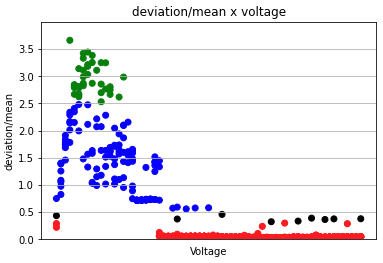
\includegraphics{Figuras/report2/data3_sjaaksgraph2.png}}
    \caption{EHDA automation system setup}
    \label{fig:sjaaks_statistical_class}
\end{figure}

 
 through statistical analysis in the signal such as mean value and standart deviation.
 Our classification by statistical analysis was implemented in the automation library made by the previous student \cite{Monica}.

 Each current sample is 0.5s of current data in 10kHz sampling frequency.
 By the processing thread we take this sample and evaluate the followings statistical values.
        
        - Sjaak Classification -> Classifies Dripping, Intermittent and Cone Jet
        
        - Monica Classification -> Classifies Corona Sparks

        - João Classification -> Classifies Multi Jet

	The algorithm implemented works in the following way:
	\begin{algorithm}
        \caption{Statistical Classification}\label{alg:statistical_class}
        \begin{algorithmic}
        \Function{statistical\_classification}{$sample$} 

            \State $spray\_mode \gets "Undefined"$;
            \State $mean \gets sample.mean$; 
            \State $std\_deviation \gets sample.std\_deviation$;
            \State $median \gets sample.median$;
            
            \If{ $mean / std\_deviation$ > 2.5}
                \Comment{Sjaak classification \cite{Sjaaks}} 
                \State $spray\_mode \gets "Dripping"$;
            \ElsIf{$ 2.5 < mean / std\_deviation < 2.5 \And mean / std\_deviation > 0.3 $}
                \State $spray\_ mode \gets "Intermittent"$;
            \ElsIf{ $mean / std\_deviation$ < 0.3}
                \State $spray\_ mode \gets "Cone Jet"$;
                \State $cone\_jet\_mean \gets mean$;
            \EndIf

            \If{ $mean / std\_deviation$ > 2.5}
                \Comment{Monica classification \cite{Monica}} 
            \EndIf

            \If{ $spray\_mode == "Cone Jet"$}
                \Comment{João classification} 
                \If{ $cone\_jet\_mean > 1.14 \times mean$}
                    \State $spray\_ mode \gets "Multi Jet"$;
                \EndIf
            \EndIf

            \Return $spray\_ mode$;
        \EndFunction
        \end{algorithmic}
    \end{algorithm}


\subsection{Machine Learning}


\section{Routine Sequences}
\label{sec:routine_sequences}

    The software was previously developed as a electrospray multipurpose library\cite{Monica}. 
    Continuing this methodology, in the setup json file there is a "sequence" atribute which can chosen beetween "ramp", "step", "map" or "control".
    The controller thread will manage what the algorithm must do for each sequence.

\subsection{Ramp}



\subsection{Step}


\begin{algorithm}
    \caption{STEP sequence in controller thread}\label{alg:stepping_algorithm}
    \begin{algorithmic}
    \Procedure{STEP}{$voltage\_start,voltage\_stop$} 
        \State $voltage \gets voltage\_start$
        \While{$voltage \leq voltage\_stop$} \Comment{scanning voltage range}
            \State \Call{send\_voltage\_command}{voltage}
            \State \Call{sleep}{step \_time}
            \State $voltage \gets voltage + step\_size$
        \EndWhile
    \EndProcedure

    \end{algorithmic}
\end{algorithm}

\subsection{Map}

    \begin{figure}[H]
        \center
        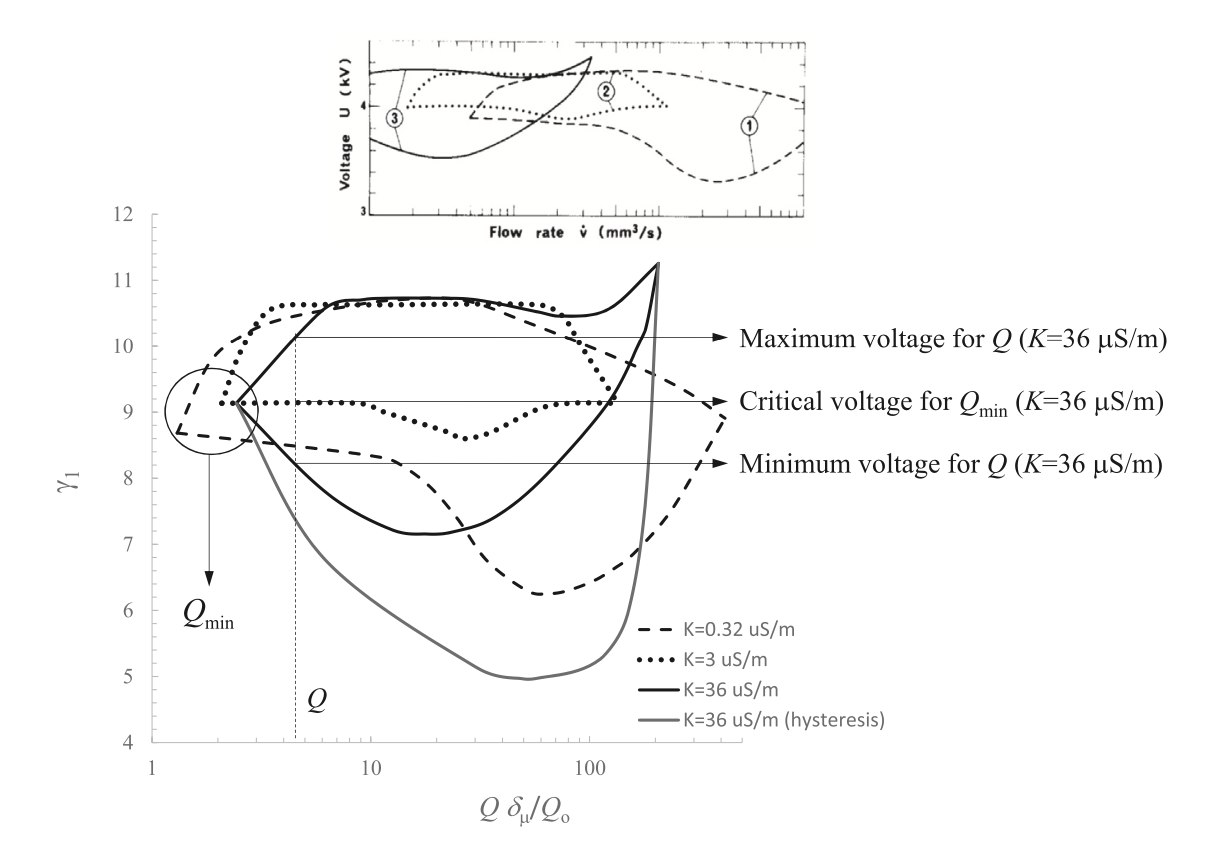
\includegraphics[width=13cm]{Figuras/ganan_calvo_map.png}
        \caption{Domains of existence (stability) of Taylor cone-jets. \cite{gananCalvo} }
        \label{fig:ganan_calvo_fig}
    \end{figure}


    \begin{algorithm}
        \caption{MAP sequence in controller thread}\label{alg:mapping_algorithm}
        \begin{algorithmic}
        \Procedure{MAP}{$flowrate\_values$} 
            \ForAll{flowrate\_values}  \Comment{scanning in the flowrate range}
                \State \Call{send\_flowrate\_command}{flowrate}
                \State $voltage \gets voltage\_start$
                \While{$voltage \leq voltage\_stop$} \Comment{scanning in the voltage range}
                    \State \Call{send\_voltage\_command}{voltage}
                    \State \Call{sleep}{step \_time}
                    \State $voltage \gets voltage + step\_size$
                \EndWhile
            \EndFor
        \EndProcedure

        \end{algorithmic}
    \end{algorithm}

    In the figures 5 and 6 we can see the results of this mapping experiments. The liquid used is pure ethanol. 
    Each figure has 3 graphs with shared x axis representing the samples collected. The first is the current values collected through all the experiment.
    The second is the voltage values applied in each window of data collected. The colors represent the spraying classification defined by our routine.
    The third graph shows the current mean value of each data sample.
    Note that the experiment is composed of loops that increase voltage, change flowrate and repeat.


    \begin{figure}[H]
        \center
        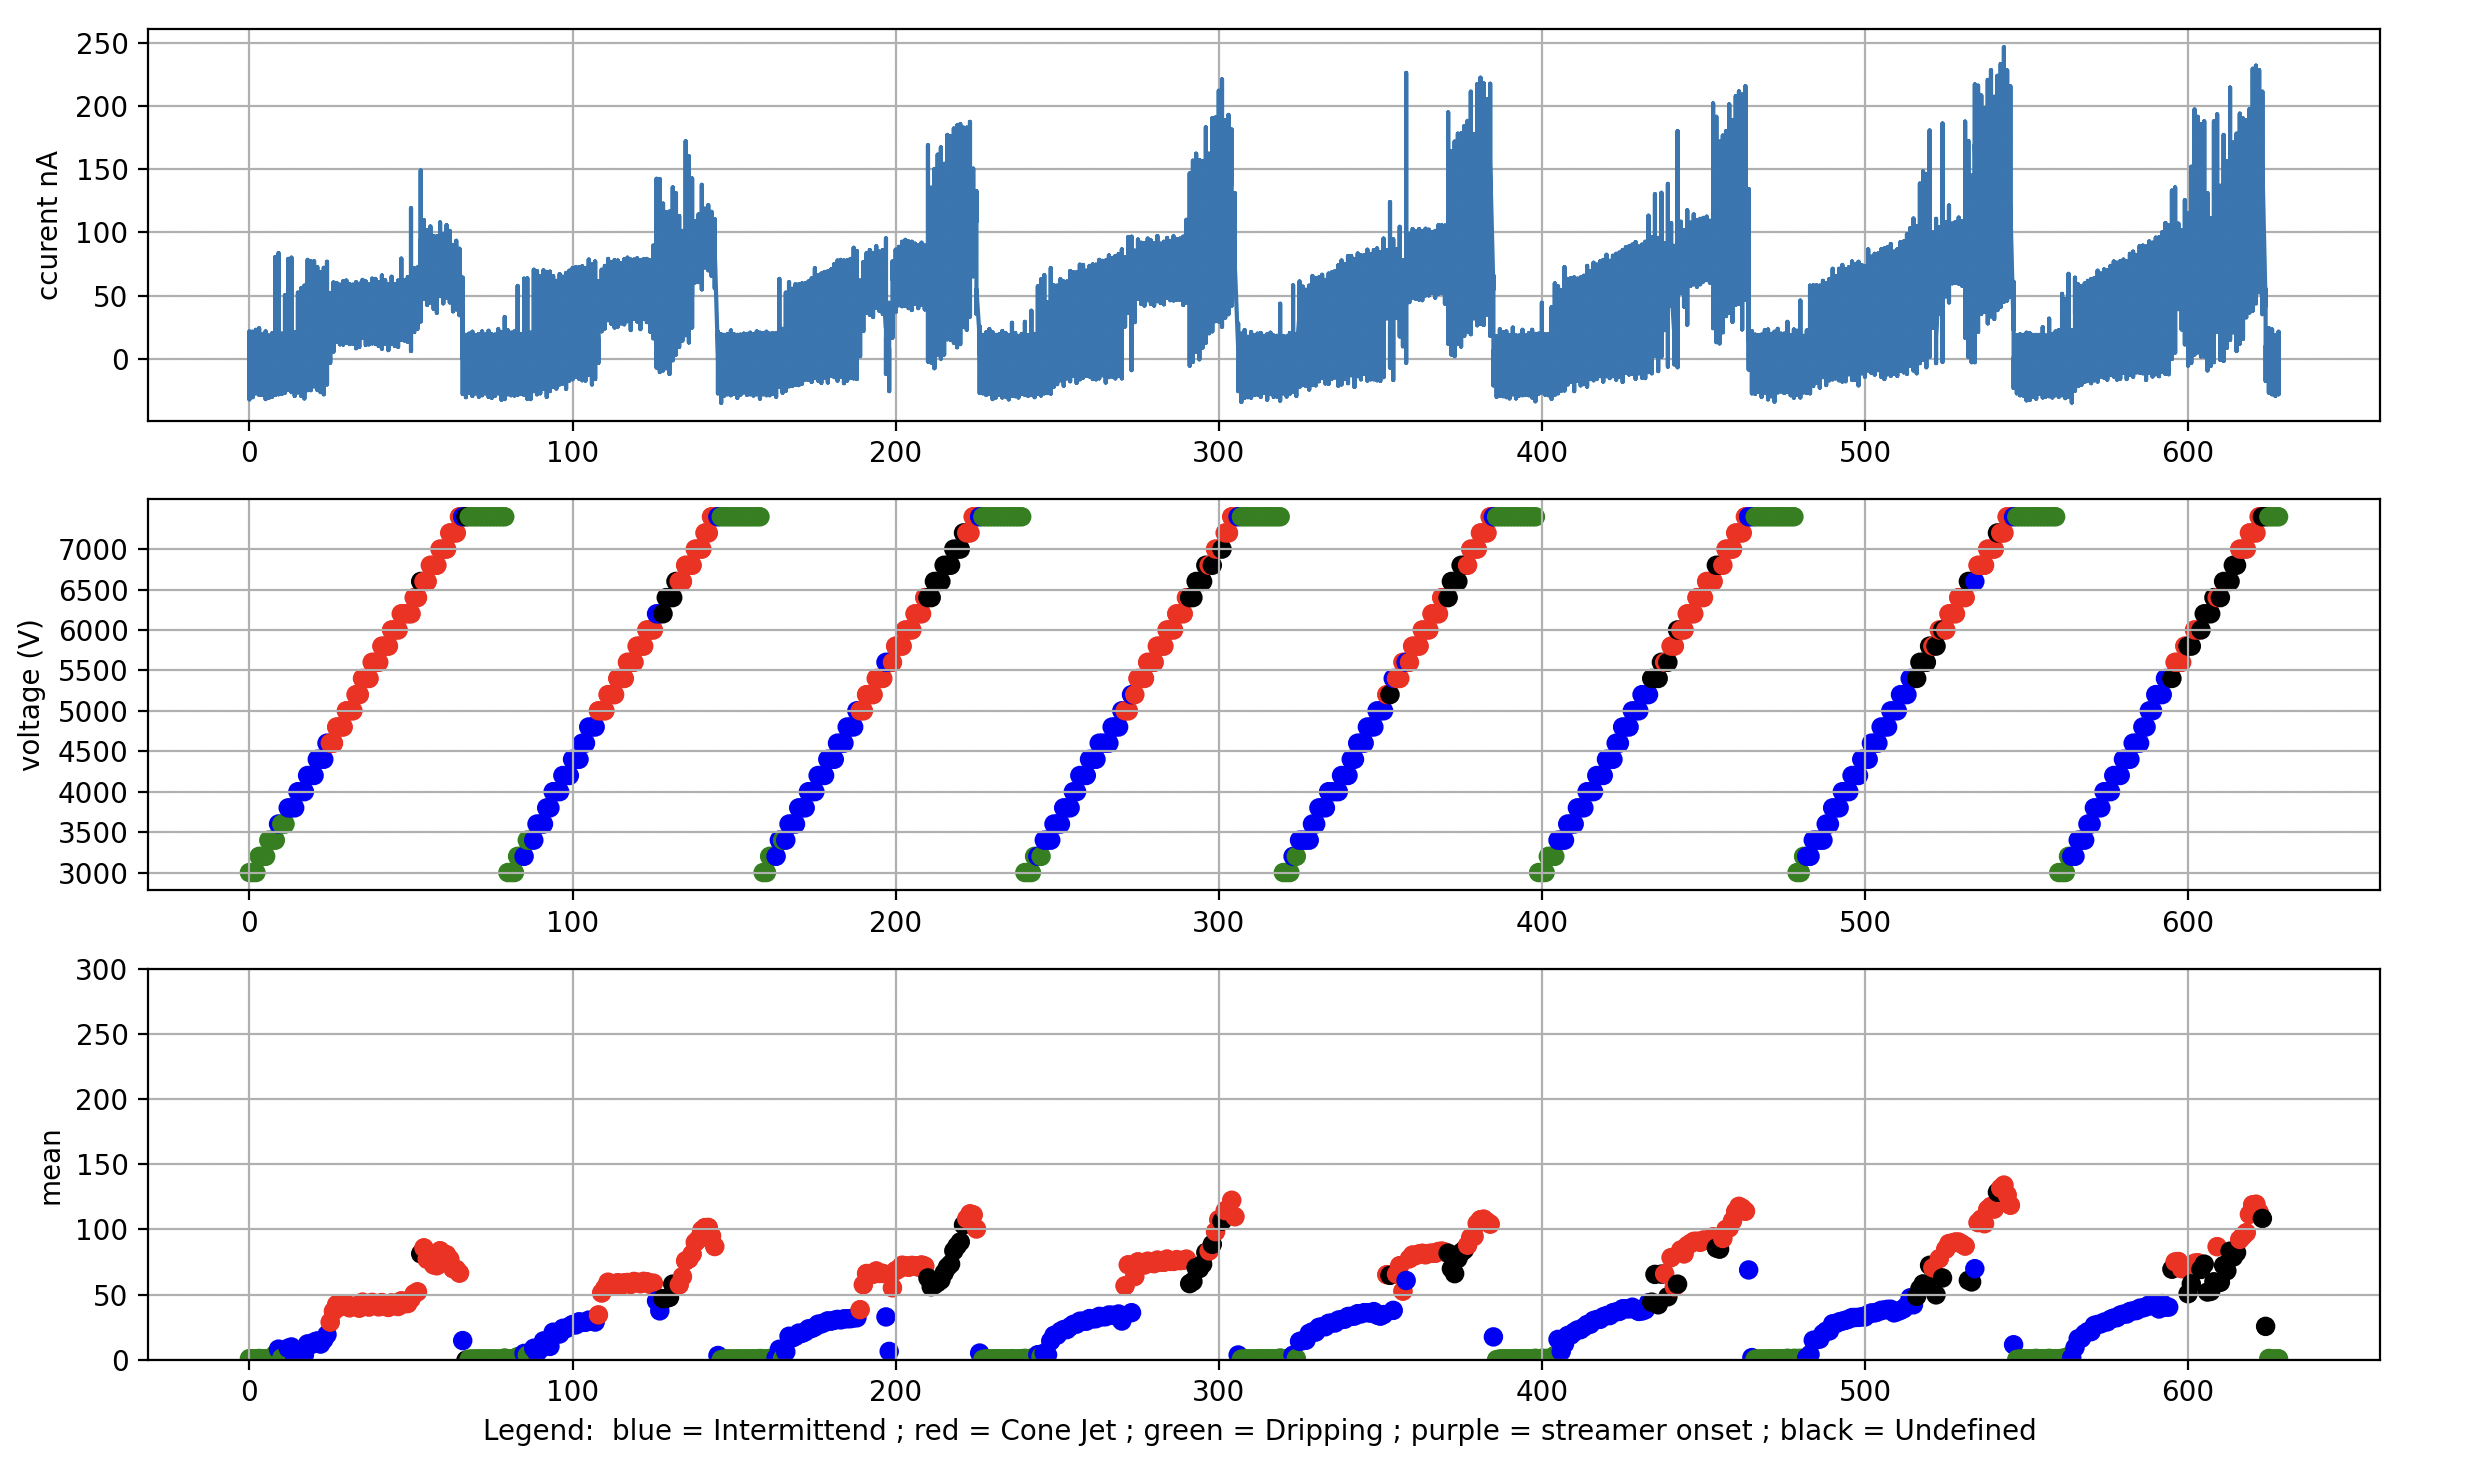
\includegraphics[width=15cm]{Figuras/report2/map2Data.png}
        \caption{Mapping Experiment example 1}
        \label{fig:map2Data_fig}
    \end{figure}


    \begin{figure}[H]
        \center
        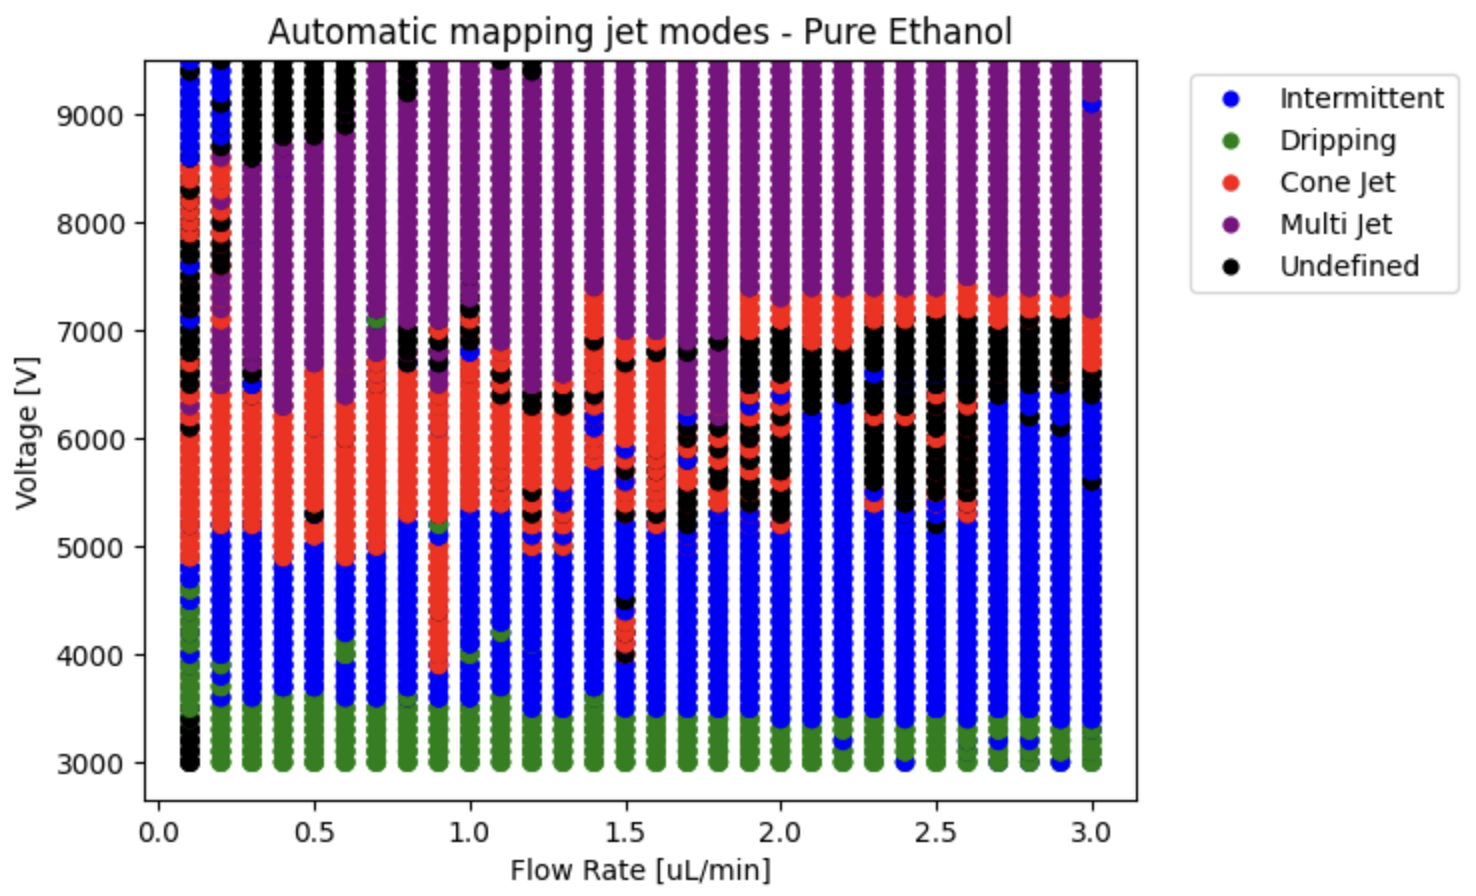
\includegraphics[width=15cm]{Figuras/report4/map-2023-03-02.png}
        \caption{Mapping Experiment example 1}
        \label{fig:map3Data_fig}
    \end{figure}



\subsection{Control}

    The control sequence is the only from our list of sequences that actually uses the feedback value. 
    As it is a closed loop control system the controller must be able to stabilize the system in the desired conditions.



\section{System Portability}
\label{sec:portability}

    Raspberry Pi


\clearpage